
\subsection{Sentence VAE}
\begin{frame}
\thetitle{Text VAE Example \citep{Bowman2016}}
Generative Model (Model 2):
\begin{itemize}
    \item Draw $\boldz \sim \mathcal{N}(\mathbf{0}, \mathbf{I})$
    \item Until end-of-sentence:
    \begin{itemize}
    %\item Set $\boldh_{\boldz,t} = \LSTM(\boldh_{\boldz,t-1}, [\boldx_{t} ; \boldz])$
    \item Draw $x_{t} \given x_{<t}, \boldz \sim \RNN([\boldh_{t-1}, \boldz] \param \theta)$
    %p(x_t \given x_{<t},\boldz \param \theta)$
    %\item Draw $x_{t+1} \given x_{<t}, \boldz \sim \softmax(\mathbf{W}\boldh_{\boldz,t})$ %p(x_t \given x_{<t},\boldz \param \theta)$
    % \[  \]
    % \[ p(x_t \given x_{<t}, \boldz ) = \softmax(\mathbf{W}\boldh_{\boldz,t-1})_{x_t}\]
    \end{itemize}
\end{itemize}

Variational Model (Amortized): Deep Diagonal Gaussians, 
\[ q(\boldz \given x \param \lambda ) = \mathcal{N}(\boldsymbol{\mu}, \boldsymbol{\sigma^2}) \]
\[ \tilde{\boldh}_T = \LSTM(x; \pi) \]
\[ \boldsymbol{\mu} = \mathbf{W}_1\tilde{\boldh}_T \,\,\,\,\,\,\,\,\,\, \boldsymbol{\sigma^2} = \exp(\mathbf{W}_2 \tilde{\boldh}_T)\]
\[ \lambda = \{\mathbf{W}_1, \mathbf{W}_2, \pi\}\]
\end{frame}


\begin{frame}
\thetitle{Text VAE Example \citep{Bowman2016}}
\center
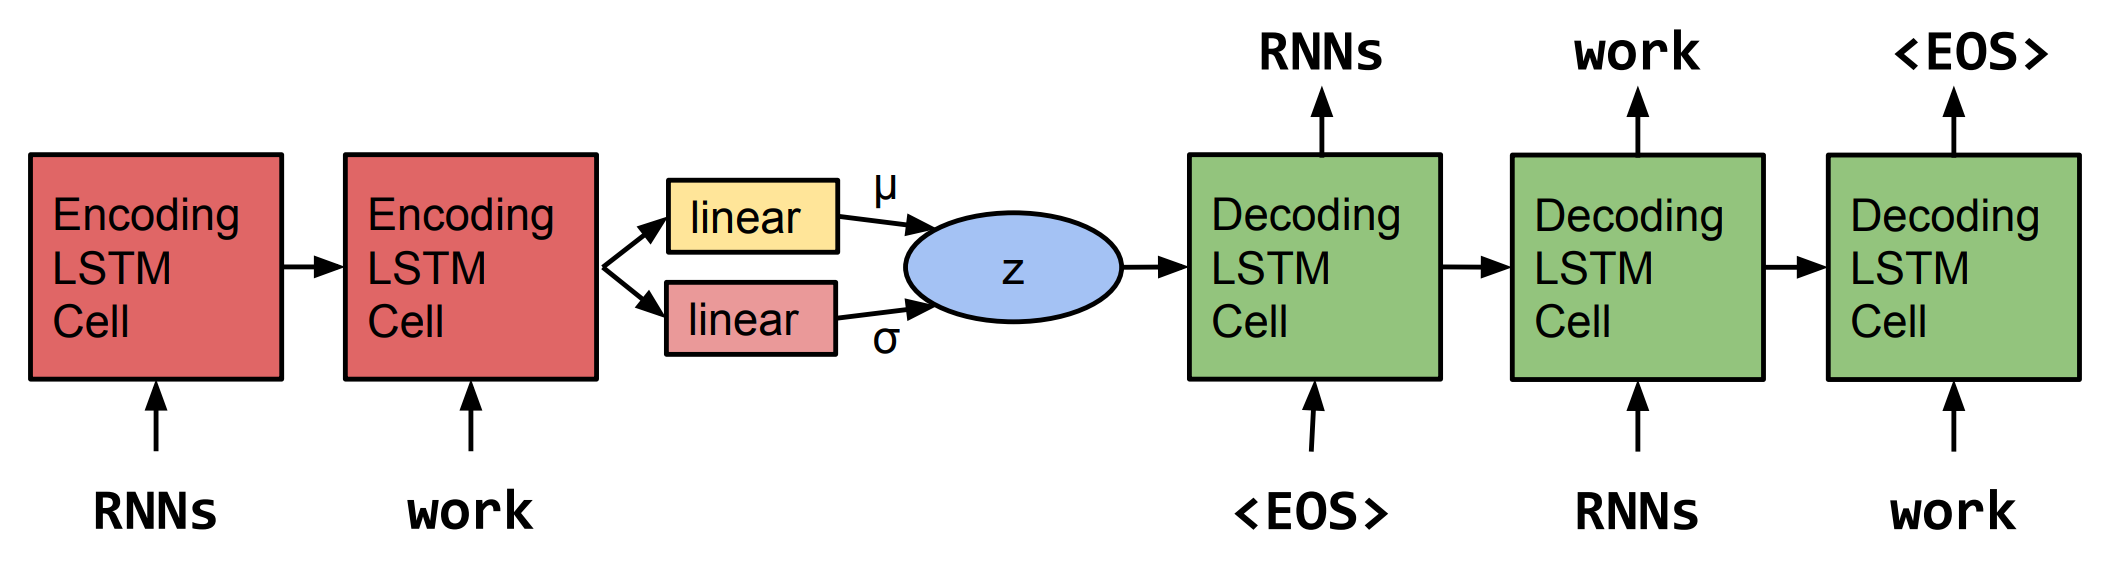
\includegraphics[scale=0.33]{pics/seq2seq_vae_text.png} \\

(from \cite{Bowman2016})

\begin{center}
\begin{tikzpicture}

     \node[latent] (zl) {$z$};%
     \node[const, below=of zl] (xl) {$x^{}$};%
     \node[const, left=of zl] (lambda) {$\lambda$};
     \edge{lambda}{zl};
     \edge{xl}{zl};
    
    \begin{scope}[xshift=5cm, yshift=-1cm]
% nodes
\node (dots) {$\ldots$};%
 \node[obs, left=1cm of dots] (x1) {$x_1^{}$};%
 \node[obs, right=1cm of dots] (xT) {$x_T^{}$};%
 \node[latent, above=5mm of dots] (z) {$z$}; %

 \edge {z} {dots};
 \edge {z} {x1};
 \edge {z} {xT};
 %\edge {mu} {z};
 %\edge {sigma} {z};
 \edge {x1} {dots};
 %\edge[bend left] {x1.south} {xT.south};
  \edge {dots} {xT};
% \edge {pi.east} {x1,xT.south};

 \draw[->] 
 (x1) edge[bend right] node [right] {} (xT);
 %\draw[->]
 %(dots) edge[bend right] node [right] {} (xT);

\end{scope}

 \node(eps)[latent,  above = 5mm of z]{$\epsilon$};
\draw (eps) edge[->] node (mid){} (z);
\draw (zl) edge[dashed]  (mid);

\end{tikzpicture}
\end{center}
\end{frame}

% \begin{frame}
% \thetitle{Text VAE Example \citep{Bowman2016}}

% Objective (for single data point):
% \begin{align*}
%     &\ELBO(\theta, \phi \param x) = \E_{q(\boldz \given x \param \phi)}\Big[\log \frac{p(x, \boldz \param \theta)}{q(\boldz \given x \param \phi)} \Big] \\
%     &= \E_{q(\boldz \given x \param \phi)}[\log p(x \given \boldz \param \theta) ] - \KL[q(\boldz \given x \param \phi) \Vert p(\boldz)]
% \end{align*}
% Gradient with regard to $\theta$: 
% \[ \nabla_\theta \ELBO(\theta, \phi \param x) = \E_{q(\boldz \given x \param \phi)}[\nabla_\theta \log p(x \given \boldz \param \theta) ]  \]
% (expectation approximated with a single sample)
% \end{frame}

% \begin{frame}
% \thetitle{Text VAE Example \citep{Bowman2016}}
% Gradient with regard to $\phi$:
% \\ First note 
% \[\KL[q(\boldz \given x \param \phi) \Vert p(\boldz)]  = -\frac{1}{2}\sum_{j=1}^d (\log \boldsymbol{\sigma}^2_j - \boldsymbol{\sigma}^2_j - \boldsymbol{\mu}_j^2 + 1) \]
% So $\nabla_\phi \KL[q(\boldz \given \boldx \param \phi) \Vert p(\boldz)]$ is easy. \\
% \[ \, \]
% Much harder:
% \[ \nabla_\phi \E_{q(\boldz \param x \param \phi)}[\log p( x \given \boldz \param \theta)]\]
% \end{frame}

% \begin{frame}
% \thetitle{Text VAE Example \citep{Bowman2016}}
% In the general case, use score function gradient estimator (aka REINFORCE \citep{Williams1992})
% \begin{align*}
%     & \nabla_\phi \E_{q(\boldz \given x \param \phi)}[\log p( x \given \boldz \param \theta)] = \nabla_\phi \int \log p(x \given \boldz \param \phi) q(\boldz \given x \param \phi)d\boldz \\
%     &= \int \log p(x \given \boldz \param \theta) \nabla_\phi q(\boldz \given x \param \phi)d\boldz \\
%      &= \int \log p(x \given \boldz \param \theta)  q(\boldz \given x \param \phi) \nabla_\phi \log  q(\boldz \given x \param \phi) d\boldz \\   
%           &=   \E_{q(\boldz \given x \param \phi)}[\log p(x \given \boldz \param \theta)  \nabla_\phi \log  q(\boldz \given x \param \phi)]
% \end{align*} 
% (since $\nabla p = p \nabla \log p$)\\

% And we can against estimate the gradient with samples from $q(\boldz \given x \param \phi)$
% \end{frame}


% \begin{frame}
% \thetitle{Text VAE Example \citep{Bowman2016}}
% The reparameterization trick: under our choice of $\mathcal{Q}$, we can draw a sample from $\boldq(\boldz \given \boldx \param \phi)$ by
% \[ \boldsymbol{\epsilon} \sim \mathcal{N}(\mathbf{0}, \mathbf{I}) \,\,\,\,\,\,\,\,\,\,\,\,\,\,\, \boldz =  \boldsymbol{\mu} + \boldsymbol{\epsilon}\boldsymbol{\sigma}\]
% Then
% \begin{align*}
%     \nabla_\phi \E_{q(\boldz \given x \param \phi)}[\log p( &x \given \boldz \param \theta)] \\  &= \nabla_\phi \E_{\epsilon \sim \mathcal{N}(\mathbf{0}, \mathbf{I})}[\log p( x \given  \boldsymbol{\mu} + \boldsymbol{\epsilon}\boldsymbol{\sigma} \param \theta)] \\
%     &= \E_{\epsilon \sim \mathcal{N}(\mathbf{0}, \mathbf{I})}[\nabla_\phi \log p(x \given  \boldsymbol{\mu} + \boldsymbol{\epsilon}\boldsymbol{\sigma} \param \theta)] 
%     \end{align*}
%     Empirically yields much lower-variance gradient estimators.
% \end{frame} 

% \begin{frame}
% \thetitle{Text VAE Example \citep{Bowman2016}}
% The reparameterization trick
% \center
% 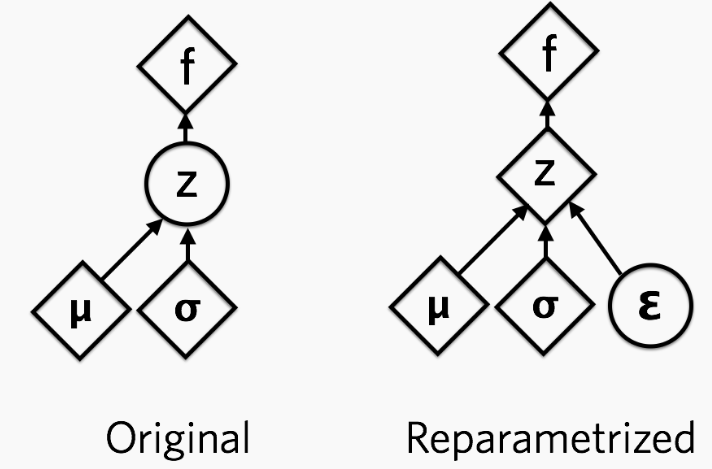
\includegraphics[scale=0.35]{pics/reparam.png}
% \end{frame} 

\begin{frame}
\thetitle{Issue: Posterior Collapse}

\begin{eqnarray*} 
\ELBO(\theta, \lambda) &= \displaystyle \E_{q(z \given x \param \lambda)}[\log \frac{p( x, z \param \theta)}{ q(z \given x \param \lambda)}] \\\\
&= \underbrace{\E_{q(z \given x \param \lambda)}[\log p( x \given z \param \theta)]
}_{\text{Reconstruction likelihood}} - \underbrace{\KL[q(z \given x \param \lambda) \Vert p(z)]}_{\text{Regularizer}} 
\end{eqnarray*}
\center

\vspace{5mm}
\begin{tabular}{l c c c }
\toprule
     Model & LL/ELBO & Reconstruction & KL \\
\midrule     
     RNN LM & -329.10 & - & - \\
     RNN VAE & -330.20 & -330.19 & 0.01 \\
\bottomrule
\end{tabular} \\
\vspace{5mm}
(On Yahoo Corpus from \cite{Yang2017}) \\
\end{frame} 

\begin{frame}
\thetitle{Issue: Posterior Collapse}
\begin{itemize}
%   \item Posterior collapse: $x$ and $z$ are independent and the generative model $p(x, z \param \theta)$
%     reduces to a standard language model (without latent variables).

  \item $x$ and $z$ become independent, and $p(x, z \param \theta)$
    reduces to a non-LV language model.    
    
    \air
    % \item \citet{Chen2017}: With a fully autoregressive/powerful likelihood model $p(x \given z \param \theta)$,    if it is possible to model $p_\star(x)$ without making use of $z$, then optimum is at
    \item \citet{Chen2017}: If it's possible to model $p_\star(x)$ without making use of $z$, then ELBO optimum is at:    
    \[ p_\star(x) = p(x \given z \param \theta) = p(x \param \theta) \]
    \[ q(z \given x \param \lambda) = p(z) \]
    \[ \KL[q(z \given x \param \lambda) \Vert p(z)] = 0\] 
\end{itemize}
\end{frame} 

\begin{frame}
\thetitle{Mitigating Posterior Collapse}
Use less powerful likelihood models~\citep{Miao2016,Yang2017},
or ``word dropout" \citep{Bowman2016}. \\
\vspace{2mm}
\center
\begin{tabular}{l c c c }
\toprule
     Model & LL/ELBO & Reconstruction & KL \\
\midrule     
     RNN LM & -329.1 & - & - \\
     RNN VAE & -330.2 & -330.2 & 0.01 \\
     $\,\,\,\,$ + Word Drop & -334.2 & -332.8 & 1.44\\
     CNN VAE & -332.1 & -322.1 & 10.0 \\ 
\bottomrule
\end{tabular} \\
\vspace{5mm}
(On Yahoo Corpus from \cite{Yang2017}) \\
\end{frame} 

\begin{frame}
\thetitle{Mitigating Posterior Collapse}
Gradually anneal multiplier on KL term, i.e.
\[\E_{q(z \given x \param \lambda)}[\log p( x \given z \param \theta)] - \beta\KL[q(z \given x \param \lambda) \Vert p(z)] \]
$\beta$ goes from 0 to 1 as training progresses
\\
\center
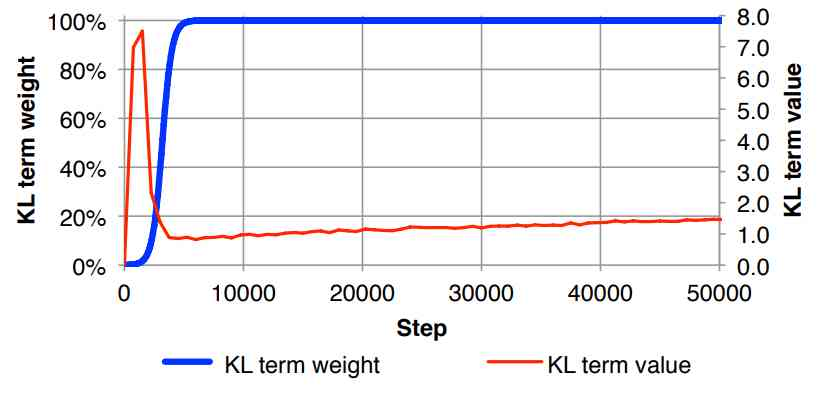
\includegraphics[scale=0.25]{kllambda.jpg}
\\
(from \cite{Bowman2016})
\end{frame} 

\begin{frame}
\thetitle{Mitigating Posterior Collapse}
Other approaches:
\begin{itemize}
    \item Use auxiliary losses (e.g. train $z$ as part of a topic model) \citep{Dieng2017,wang2017topic}
    \item Use von Mises--Fisher distribution with a fixed concentration parameter  \citep{Guu2017,xu2018}
    \item Combine stochastic/amortized variational inference \citep{Kim2018}
    \item Add skip connections \citep{dieng2018}
\end{itemize}
\air
\air
In practice, often necessary to combine various methods.
\end{frame} 

\begin{frame}
\thetitle{Issue: Evaluation}
\begin{itemize}
    \item ELBO always lower bounds $\log p(x \param \theta)$, so can calculate an upper bound on PPL efficiently.
    \item When reporting ELBO, should also separately report
    \[ \KL[q(z \given x \param \lambda) \Vert p(z)] \] 
    to give an indication of how much the latent variable is being ``used".
\end{itemize}
\end{frame} 

\begin{frame}
\thetitle{Issue: Evaluation}
    
    Also can evaluate $\log p(x \param \theta)$ with importance sampling
    \begin{align*}
        p(x \param \theta) &= \E_{q(z \given x \param \lambda)}\Big[\frac{p(x \given z \param \theta)p(z)}{q(z \given x \param \lambda)}\Big] \\
        &\approx \frac{1}{K}\sum_{k=1}^K \frac{p(x | z^{(k)} \param \theta)p(z^{(k)})}{q(z^{(k)} \given x \param \lambda)}
    \end{align*}
    So 
    \[ 
    \implies \log p(x \param \theta) \approx \log \frac{1}{K}\sum_{k=1}^K \frac{p(x | z^{(k)} \param \theta)p(z^{(k)})}{q(z^{(k)} \given x \param \lambda)}
\]
%(biased but consistent estimator)
\end{frame} 

\begin{frame}
\thetitle{Evaluation}
Qualitative evaluation 
\begin{itemize}
    \item Evaluate samples from prior/variational posterior. 
    \item Interpolation in latent space. 
\center
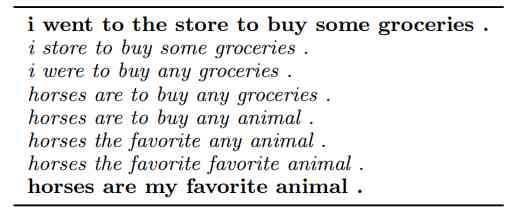
\includegraphics[scale=0.5]{pics/zinterp.jpg} \\
(from \cite{Bowman2016})
\end{itemize}
\end{frame} 

\subsection{Encoder/Decoder with Latent Variables}

\newcommand{\benc}{\boldsymbol{\mathrm{enc}}}

\begin{frame}
\thetitle{Encoder/Decoder ~\citep{Sutskever2014,Cho2014b}}
\begin{center}
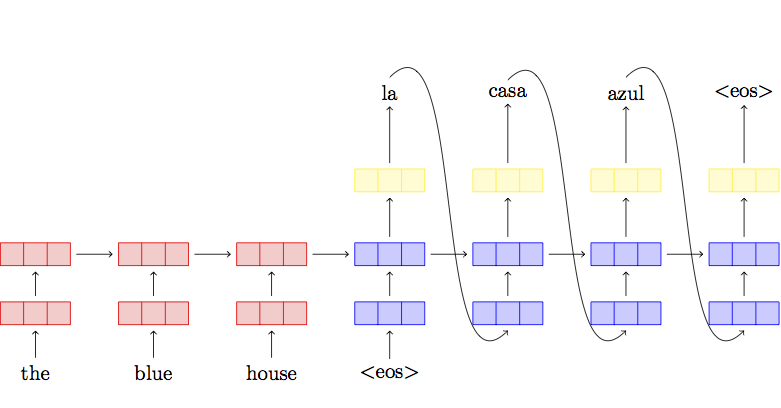
\includegraphics[scale=0.55]{pics/seq2seq.png}
\end{center}

\textbf{Given:} Source information $s = s_1, \ldots, s_M$.
\air

\textbf{Generative process:} For words $t=1, \ldots, T$
  \begin{itemize}
     %\item Set $\boldh_t = \RNN(\boldh_{t-1}, [\boldx_t, \benc(s)])$.
      \item Draw $x_{t} \given x_{< t}, s \sim \RNN([\boldh_{t-1}, \benc(s)] \param \theta)$.
  \end{itemize}




\air
%Log likelihood: 
$ \implies  p(x_{1:T} \given s \param \theta) =  \prod_{t=1}^T \RNN([ \boldh_{t-1}, \benc(s)])_{x_t}$.
    % \begin{align*}
    %     \log p(x_{1:T} \given s \param \theta) = \log \prod_{t=1}^T \softmax(\boldW \boldh_{t-1})_{x_t}.
    % \end{align*}
    % \begin{align*}
    %     p(x_1, \ldots, x_T \given s \param \theta) &= \prod_{t=1}^T p(x_t \given x_{<t}, s \param \theta) \\
    %     &= \prod_{t=1}^T \softmax(\boldW \boldh_{t-1})_{x_t},
    % \end{align*}
\end{frame}

\begin{frame}
\thetitle{Latent, Per-token Experts~\citep{yang2018breaking}}

\textbf{Generative process:} For $t=1, \ldots, T$,
\begin{itemize}
    %\item Set $\boldh_t = \RNN([\boldx_t, \benc(s)], \boldh_{t-1})$.
    \item Draw $z_{t} \given x_{< t}, s \sim \text{Cat}(\softmax(\boldU \boldh_{t-1}))$.
    \item Draw $x_{t} \given z_{t}, x_{< t}, s \sim \RNN(\tanh(\boldQ_{z_t} \boldh_{t-1}) \param \theta)$ %\text{Cat}(\softmax(\boldW \tanh(\boldQ_{z_t} \boldh_t)))$.
\end{itemize}
\begin{center}

\begin{tikzpicture}
  %\tikz{
% nodes
\node (dots) {$\ldots$};%
 \node[obs, left=1cm of dots] (x2) {$x_2^{(n)}$};%
 \node[obs, left=1cm of x2] (x1) {$x_1^{(n)}$};%
 \node[obs, right=1cm of dots] (xT) {$x_T^{(n)}$};%
 \node[latent, above=of x1] (z1) {$z_1^{(n)}$}; %
 \node[latent, above=of x2] (z2) {$z_2^{(n)}$}; %
 \node[latent, above=of xT] (zT) {$z_T^{(n)}$}; %
 %\node[const, above=(0.5cm) of z] (mu) {$\mu$};
 %\node[const, below left=0.3cm and 0.8cm of x1] (pi) {$\pi$};
 
% plate
 \plate {plate1} {(dots)(x1)(x2)(xT)(z1)(z2)} {$N$}; %
% edges

 \edge {x1} {zT};
 \edge {x2} {zT};
 \edge {dots} {zT};
 
 \edge {x1} {z2};

 \edge {z1} {x1};
 \edge {z2} {x2};
 \edge {zT} {xT};
 %\edge {mu} {z};
 %\edge {pi.east} {x1,xT.south};
 \edge {x1} {x2};
 \edge {x2} {dots};
 %\edge[bend left] {x1.south} {xT.south};
  \edge {dots} {xT};

 \draw[->] 
 (x1) edge[bend right=20] node [right] {} (xT);
 %}
 \end{tikzpicture}
 %}
\end{center}
\air 
\air
If $\boldU \in \reals^{K \times d}$, we have $K$ experts; increases the flexibility of the per-token distribution.



\end{frame}

\begin{frame}
\thetitle{Latent, Per-token Experts~\citep{yang2018breaking}}
\textbf{Learning:} $z_t$ are independent given $x_{<t}$, so we can marginalize at each time-step (coordinate ascent).
    \begin{align*}
        &\argmax_{\theta} \log p(x \given s \param \theta) =  \\
        &\argmax_{\theta} \log \prod_{t=1}^T \sum_{k=1}^K p(z_t {=} k \given s, x_{<t} \param \theta) p(x_t \given z_t{=}k, x_{<t}, s \param \theta).
    \end{align*}

\textbf{Test-time:}
\begin{align*}
\argmax_{x_{1:T}} \prod_{t=1}^T \sum_{k=1}^K p(z_t {=} k \given s, x_{<t} \param \theta) p(x_t \given z_t{=}k, x_{<t}, s \param \theta)
\end{align*}
\end{frame}

\begin{frame}
    \thetitle{Latent, Per-token Experts~\citep{yang2018breaking}}
PTB language modeling results ($s$ is constant):
\air
\begin{table}
\begin{tabular}{lc}
\toprule
     Model & PPL \\
\midrule     
     \citet{merity2018regularizing} & 57.30 \\
     Softmax-mixture~\citep{yang2018breaking} & 54.44 \\
\bottomrule
\end{tabular}  
\end{table}

\air
\air
        
Dialogue generation results ($s$ is context):
\air
\begin{table}
\begin{tabular}{lcc}
\toprule
     Model &  \multicolumn{2}{c}{BLEU} \\
     & Prec & Rec \\
\midrule     
     No mixture & 14.1 & 11.1 \\
     Softmax-mixture~\citep{yang2018breaking} & 15.7 & 12.3 \\
\bottomrule
\end{tabular}
\end{table}
    
\end{frame}

\begin{frame}
\thetitle{Attention~\citep{Bahdanau2015}}
\begin{center}
    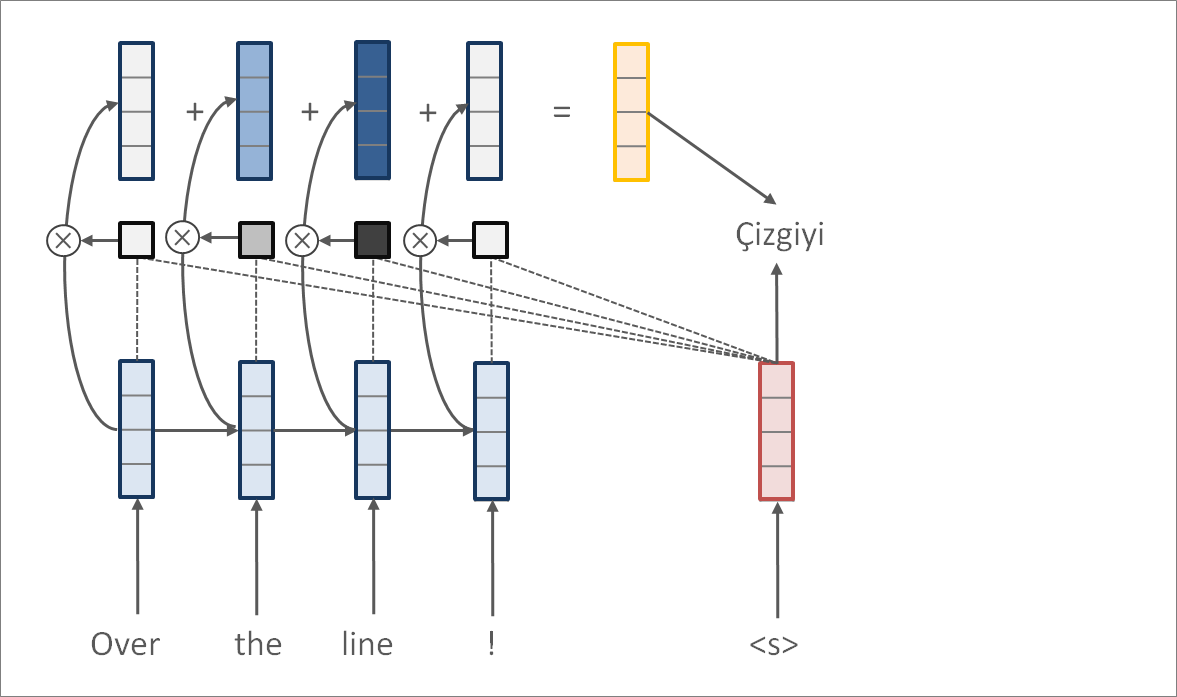
\includegraphics[scale=0.24]{pics/attn1step.png}
\end{center}

Decoding with an attention mechanism:

\[p(x_{t} \given x_{< t}, s \param \theta) = \RNN([\boldh_{t-1}, {\sum_{m=1}^M} \alpha_{t,m} \,  \benc(s_m)])_{x_{t}}.\]


% \air
% \begin{itemize}
%     \item Learning the same as in standard encoder/decoder.
% \end{itemize}

\end{frame}

\begin{frame}
\thetitle{Copy Attention}
Copy attention~\citep{gu2016incorporating,gulcehre2016pointing} models copying words directly from $s$.
\air

\textbf{Given:} Source information $s = s_1, \ldots, s_M$.
\air

\textbf{Generative process:} For $t=1, \ldots, T$,
\begin{itemize}
    %\item Set $\boldh_t = \RNN([\boldx_t, \benc(s)], \boldh_{t-1})$.
    \item Set $\balpha_t$ to be attention weights.
    \item Draw $z_{t} \given x_{< t}, s \sim \mathrm{Bern}(\MLP([\boldh_{t-1}, \benc(s)]))$.
    \item If $z_{t} = 0$
    \begin{itemize}
        \item Draw $x_{t} \given z_{t}, x_{< t}, s \sim \RNN(\boldh_{t-1} \param \theta)$.
    \end{itemize}
    \item Else 
    \begin{itemize}
        \item Draw $x_{t} \in \{s_1, \ldots, s_M\} \given z_{t}, x_{< t}, s \sim \mathrm{Cat}(\balpha_t)$.

    \end{itemize}
    \end{itemize}

\end{frame}

\begin{frame}
\thetitle{Copy Attention}
\textbf{Learning:} Can maximize the log per-token marginal~\citep{gu2016incorporating}, as with per-token experts:
        \begin{align*}
        &\max_{\theta} \log p(x_1, \ldots, x_T \given s \param \theta) \\
        = &\max_{\theta} \log \prod_{t=1}^T \sum_{z' \in\{0, 1\}} p(z_t = z' \given s, x_{<t} \param \theta) p(x_t \given z', x_{<t}, x \param \theta).
    \end{align*}
    
    \air
    \air
\textbf{Test-time:}
\begin{align*}
\argmax_{x_{1:T}} \prod_{t=1}^T \sum_{z' \in\{0, 1\}} p(z_t {=} z' \given s, x_{<t} \param \theta) p(x_t \given z', x_{<t}, s \param \theta).
\end{align*}
\end{frame}

\begin{frame}
\thetitle{Attention as a Latent Variable~\citep{deng2018}}
\textbf{Given:} Source information $s = s_1, \ldots, s_M$.
\air

\textbf{Generative process:} For $t=1, \ldots, T$,
\begin{itemize}
    %\item Set $\boldh_t = \RNN([\boldx_t, \benc(s)], \boldh_{t-1})$.
    \item Set $\balpha_t$ to be attention weights.
    \item Draw $z_{t} \given x_{ < t}, s \sim \mathrm{Cat}(\balpha_t)$.
    \item Draw $x_{t} \given z_{t}, x_{< t}, s \sim \RNN([\boldh_t, \benc(s_{z_{t}})] \param \theta)$.
\end{itemize}

% \air
% \air
% Note $\bolda_t \in \Delta^{M-1}$.
\end{frame}

\begin{frame}
\thetitle{Attention as a Latent Variable~\citep{deng2018}}
Marginal likelihood under latent attention model:
    \begin{align*}
       p(x_{1:T} \given s \param \theta) = \prod_{t=1}^T \sum_{m=1}^M \alpha_{t,m} \RNN([\boldh_t, \benc(s_{m})] \param \theta)_{x_t}.
    \end{align*}
    
\air
\air
\air
\air

Standard attention likelihood:
    \begin{align*}
        p(x_{1:T} \given s \param \theta) = \prod_{t=1}^T  \RNN([\boldh_t, \sum_{m=1}^M \alpha_{t,m} \, \benc(s_{m})] \param \theta)_{x_t}.
    \end{align*}
    
% \air
% \air
% Only the former corresponds to the marginal likelihood of a latent variable model.
\end{frame}

\begin{frame}
\thetitle{Attention as a Latent Variable~\citep{deng2018}}
\textbf{Learning Strategy \#1:} Maximize the log marginal via enumeration as above.

\air

\textbf{Learning Strategy \#2:} Maximize the ELBO with AVI:

\begin{align*}
    \max_{\lambda, \theta} \E_{q(z_t \param \lambda)} \left[ \log p(x_t \given x_{<t}, z_t, s) \right] - \KL[q(z_t \param \lambda) \Vert p(z_t \given x_{<t}, s)].
\end{align*}

\air

\begin{itemize}
    \item $q(z_t \given x \param \lambda)$ approximates $p(z_t \given x_{1:T}, s \param \theta)$; implemented with a BLSTM.
    \item $q$ isn't reparameterizable, so gradients wrt $\lambda$ obtained using REINFORCE + baseline.
\end{itemize}

\end{frame}


\begin{frame}
\thetitle{Attention as a Latent Variable~\citep{deng2018}}
\textbf{Test-time:} Calculate $p(x_t \given x_{<t}, s \param \theta)$ by summing out $z_t$.

\air
\air
MT Results on IWSLT-2014:
\begin{table}
\begin{tabular}{lcc}
\toprule
     Model & PPL & BLEU\\
\midrule     
     Standard Attn & 7.03 & 32.31 \\
     Latent Attn (marginal) & 6.33 & 33.08 \\ 
     Latent Attn (ELBO) & 6.13 & 33.09 \\
\bottomrule
\end{tabular}
\end{table}
\end{frame}

\begin{frame}
\thetitle{Encoder/Decoder with Structured Latent Variables}
At least two EMNLP 2018 papers augment encoder/decoder text generation models with \textit{structured} latent variables:

\begin{enumerate}
    \item \citet{lee2018deterministic} generate $x_{1:T}$ by iteratively refining sequences of words $z_{1:T}$.
    \air
    \air 
    \item \citet{wiseman2018learning} generate $x_{1:T}$ conditioned on a latent template or plan $z_{1:S}$.
\end{enumerate}
    
\end{frame}

\subsection{Latent Summaries}

\begin{frame}
\thetitle{Summary as a Latent Variable~\citep{miao2016language}}
Generative process for a document $x = x_1, \ldots, x_T$:
\begin{itemize}
    \item Draw a latent summary $z_1, \ldots, z_{M} \sim p(z_1, \ldots, z_{M} \param \theta)$
    \item Draw $x_1, \ldots, x_{T} \given z_{1:M} \sim p(x_1, \ldots, x_T \given z_{1:M} \param \theta)$
    \item ($p(z \param \theta)$ and $p(x \given z \param \theta)$ modeled with encoder/decoder RNNs).
\end{itemize}

% \air
% \air
% \citet{miao2016language} parameterize prior $p(z)$ with an RNN, and generative model $p(x \given z)$ with encoder/decoder RNNs.
    
\air
\air
\air
\pause
\textbf{Note:} previously we cared most about the model generating $x_{1:T}$; here we care most about \textit{inference}: 
\begin{align*}
p(z_{1:M} \given x_{1:T} \param \theta) = p(\text{summary} \given \text{document} \param \theta).    
\end{align*}
\end{frame}

\begin{frame}
\thetitle{Summary as a Latent Variable~\citep{miao2016language}}
\textbf{Learning:} Maximize the ELBO with AVI:

\begin{align*}
    \max_{\lambda, \theta} \E_{q(z_{1:M} \param \lambda)} &\left[\log p(x_{1:T} \given z_{1:M} \param \theta) \right] \\
    &- \KL[q(z_{1:M} \param \lambda) \Vert p(z_{1:M} \param \theta)]
\end{align*}

\begin{itemize}
    \item $q(z_{1:M} \param \lambda)$ approximates $p(z_{1:M} \given x_{1:T} \param \theta)$; also implemented with encoder/decoder RNNs.
    \item $q(z_{1:M} \param \lambda)$ not reparameterizable, so gradients wrt $\lambda$ use REINFORCE + baselines.
\end{itemize}

\end{frame}

\begin{frame}
\thetitle{Summary as a Latent Variable~\citep{miao2016language}}
\textbf{Semi-supervised Training:} Can also use documents \textit{without} corresponding summaries in training.
\begin{itemize}
    \item Train $q(z_{1:M} \param \lambda) \approx p(z_{1:M} \given x_{1:T} \param \theta)$ with labeled examples.
    \air
    \item Infer summary $z$ for an \textit{unlabeled} document with $q$.
    \air
    \item Use inferred $z$ to improve model $p(x_{1:T} \given z_{1:M} \param \theta)$.
    \air
    \item Allows for outperforming strictly supervised models!
\end{itemize}
\end{frame}

\subsection{Deep Topic Models}

\begin{frame}
\thetitle{Topic Models~\citep{blei2003latent}}

\begin{center}
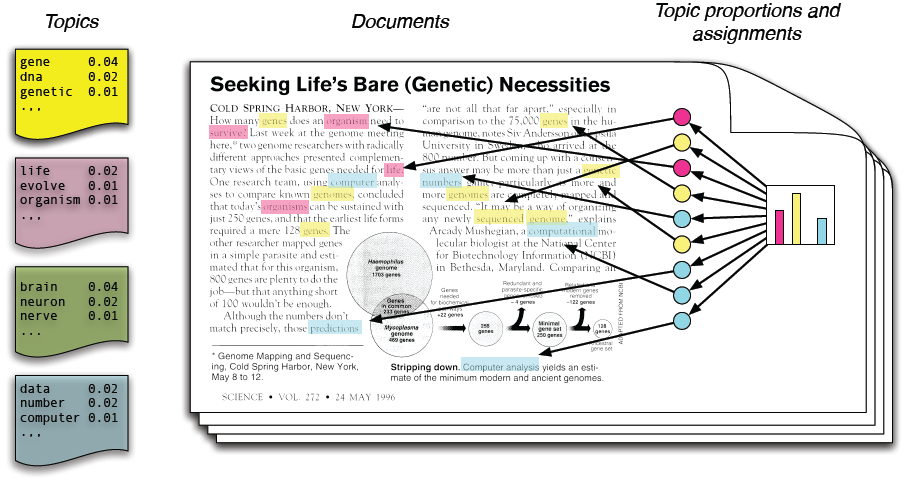
\includegraphics[scale=0.27]{pics/IntroToLDA.png}
\end{center}

Generative process: for each document $x^{(n)} = x^{(n)}_1, \ldots, x^{(n)}_T$,

\vspace{-2mm}
\begin{itemize}
    \item  Draw topic distribution $\boldz^{(n)}_{top} \sim Dir(\balpha)$
    \item  For $t=1, \ldots, T$:
    \begin{itemize}
        \item Draw topic $z^{(n)}_t \sim Cat(\boldz^{(n)}_{top})$
        \item Draw $x_t \sim Cat(\bbeta_{z^{(n)}_t})$
    \end{itemize}
\end{itemize}
    
\end{frame}

\begin{frame}
\thetitle{Simple, Deep Topic Models~\citep{miao2017nvi}}
\textbf{Motivation:} easy to learn deep topic models with AVI if $q(\boldz^{(n)}_{top} \param \lambda)$ is reparameterizable.

\air
\air
\air
\textbf{Idea:} draw $\boldz^{(n)}_{top}$ from a transformation of a Gaussian.
\begin{itemize}
    \item Draw $\boldz^{(n)}_0 \sim \mcN(\bmu_0, \bsigma^2_0)$
    \item Set $\boldz^{(n)}_{top} = \softmax(\boldW \boldz^{(n)}_0)$. %, or to an even more complicated function of $\boldz^{(n)}_0$.
    \item Use analogous transformation when drawing from $q(\boldz^{(n)}_{top} \param \lambda)$.
    
\end{itemize}
    
\end{frame}


\begin{frame}
\thetitle{Simple, Deep Topic Models~\citep{miao2017nvi}}
\textbf{Learning Step \#1:} Marginalize out per-word latents $z^{(n)}_t$. 

\begin{align*}
    p(\{x^{(n)}\}_{n=1}^N, \{\boldz^{(n)}_{top}\}_{n=1}^N \param \theta) = \prod_{n=1}^N p(\boldz^{(n)}_{top} \given \theta) \prod_{t=1}^T \sum_{k=1}^K z^{(n)}_{top, k} \, \beta_{k, x^{(n)}_t}
\end{align*}

\air
\air
\textbf{Learning Step \#2:} Use AVI to optimize resulting ELBO.
\begin{align*}
    \max_{\lambda, \theta} \E_{q(\boldz^{(n)}_{top} \param \lambda)} &\left[\log p(x^{(n)} \given \boldz^{(n)}_{top}  \param \theta) \right] \\
    &- \KL[ \mcN(\boldz^{(n)}_0 \param \lambda) \Vert \mcN(\boldz^{(n)}_0 \param \bmu_0, \bsigma_0^2)]
\end{align*}
\end{frame}


\begin{frame}
\thetitle{Simple, Deep Topic Models~\citep{miao2017nvi}}
Perplexities on held-out documents, for three datasets:

\begin{table}
\begin{tabular}{lccc}
\toprule
     Model & MXM & 20News & RCV1 \\
\midrule     
     OnlineLDA~\citep{hoffman2010online} & 342 & 1015 & 1058 \\
     AVI-LDA~\citep{miao2017nvi} & 272 & 830 & 602 \\
\bottomrule
\end{tabular}
\end{table}
\end{frame}